
\label{chapter:dthreads}

As described in Section~\ref{sec:nondeterminism}, non-determinism can greatly complicate the reasoning and debugging of parallel programs. To resolve this problem, several recent software-only proposals aim at providing deterministic multithreading. However, all of these existing approaches suffer from a variety of disadvantages. Language-based approaches are effective at removing non-determinism but require programmers to write code in specialized languages, which can be impractical~\cite{Bocchino:2009:TES:1640089.1640097,Burckhardt:2010:CPR:1869459.1869515,Simpson:1999:SEE:330346.330357}. Recent deterministic systems that target legacy programming languages (especially C/C++) are either incomplete or impractical. Kendo ensures determinism of synchronization operations with low overhead, but does not guarantee determinism in the presence of data races~\cite{1508256}. Grace prevents all concurrency errors but is limited to fork-join programs, and although it is efficient, it requires code modifications to avoid large runtime overhead~\cite{grace}. CoreDet, a compiler and runtime system, enforces deterministic execution for arbitrary multithreaded C/C++ programs~\cite{Bergan:2010:CCR:1736020.1736029}. However, it exhibits prohibitively high overhead (running up to $8\times$ slower than \pthreads{}; see Section~\ref{sec:dthreadsevaluation}) and generates thread interleavings at arbitrary points in the code, complicating program reasoning, debugging, and testing.

\hspace{1em} \\
\noindent
\textbf{Contributions:}
We develop \textbf{\dthreads{}}, an efficient deterministic runtime system for multithreaded C/C++ applications. \dthreads{} guarantees deterministic execution of multithreaded programs even in the presence of data races (notwithstanding external sources of non-determinism like I/O): given the same sequence of inputs, a program using \dthreads{} always produces the same output. \dthreads{}'s deterministic commit protocol not only eliminates data races but also prevents lock-based deadlocks.

\dthreads{} is easy to deploy: it works as a direct replacement for the \pthreads{} library, requiring no code modifications or
recompilation. \dthreads{} is also very efficient. \dthreads{} leverages process isolation and virtual memory protection to track and isolate concurrent memory updates, based on the \sheriff{} framework. Not only does this approach greatly reduce overhead, comparing to approaches that track memory reads and writes, it also eliminates cache-line based false sharing, a notorious performance problem for multithreaded
programs. These two features combine to enable \dthreads{} to nearly match or even exceed the performance of \pthreads{} for the majority of benchmarks examined here. \dthreads{} thus marks a significant improvement over the state-of-the-art in deployability and performance, and provides promising evidence that fully deterministic multithreaded programming may be practical.

\section{\dthreads{} Overview}
Figure~\ref{fig:nondeterminism} shows an example multithreaded program that, because of data races, non-deterministically produces the outputs: ``1,0,'' ``0,1,'' and ``1,1.''  The order of instructions are changed from one execution to the other, resulting in these nondeterministic outputs. Using \dthreads{}, this program will \emph{deterministically} produce the same output ``1,1.'' Although this output can be a undesired one, the fact that results are always reproducible would make it easy for developers to reproduce and locate data races inside parallel programs.

\begin{figure}[h]
{\centering
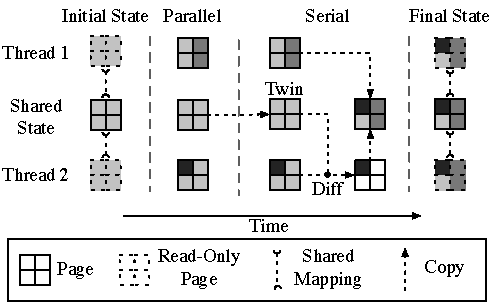
\includegraphics[width=6in]{dthreads/figure/architecture-diagram}
\caption{An overview of \dthreads{} execution.\label{fig:architecture}}
}
\end{figure}

\dthreads{} employs the following mechanisms to ensure the deterministic execution, illustrated by Figure~\ref{fig:architecture}: 

\textbf{Isolated Memory Access:} Based on the \sheriff{} framework, \dthreads{} runs threads as separate processes with private and shared views of memory, thus isolating executions of different ``threads.'' \dthreads{} uses this isolation mechanism to control the visibility of memory state, so that updates made by a thread cannot be seen by other threads if those updates are not committed explicitly to the shared mapping. By doing this, we guarantee that each ``thread'' can operate independently until synchronization points. Implementations are discussed in depth in Section~\ref{sec:threadsasprocs}.

\textbf{Deterministic Memory Commit:} 
Multithreaded programs use shared memory for communication, thus \dthreads{} must make a thread's changes seen by other threads. To guarantee determinism, \dthreads{} should publish updates of different threads in a deterministic order at deterministic points.

\dthreads{} actually commits the changes of a thread to the shared state in sequence at synchronization points. These points includes thread creation and exit; mutex lock and unlock; condition variable wait and signal; posix sigwait and signal; and barrier waits. Commits are ordered using a global token that is passed from one thread to the next; a thread can only commit when it holds the token.  The token-passing protocol is described in Section~\ref{sec:schedule} and the implementation of synchronization primitives is described in Section~\ref{sec:synchronization}.

\dthreads{} relies on the twinning-and-diffing mechanism to find out local changes of different threads, which has been discussed in Section~\ref{sec:twinning-and-diffing}. 

\textbf{Deterministic Synchronization:}
There is no deterministic guarantee on synchronizations under existing operating systems. Thus, \dthreads{} re-implements the full range of pthreads synchronization primitives and discusses  them in details in Section~\ref{sec:synchronization}. 

\hspace{1em} \\
\noindent
\textbf{Fixing the data race example} \\
About the example program in Figure~\ref{fig:nondeterminism},  \dthreads{} effectively isolates the execution from each thread until it completes, and then orders updates from different threads by thread creation time using a deterministic last-writer-wins protocol.

In the beginning of every execution, thread 1 and thread 2 have the same view of shared state, with a = 0 and b = 0. Since changes by one thread to the value of a or b are not visible to the other until this thread exits, both checks on two threads at line 2 will be true. So thread 1 sets the value of a to 1, and thread 2 sets the value of b to 1. These threads then commit their updates to the shared state and exit, with thread 1 always committing before thread 2. The main thread then should always print ``1, 1'' on every execution.

Determinism not only enables replay-without-recording and replicated executions, but also effectively converts ``Heisenbugs'' into ``Bohr'' bugs, making them reproducible. In addition, \dthreads{} optionally reports any conflicting updates due to racy writes, further simplifying debugging.


\section{\dthreads{} Architecture}

\begin{comment}
Because multithreaded programs frequently use updates to shared memory to communicate, \dthreads{} must implement a mechanism to expose one thread's updates to all other threads.  At the beginning of a transaction, all shared pages are protected, and can only be read by threads.  When a thread attempts to modify a shared page a local working copy is created, leaving the shared page unmodified.  At commit time, a ``twin'' copy of all modified pages is created.  Every page is compared to its twin (using a byte-wise diff) and modified bytes are copied back to the shared state.  Unlike transactional memory, conflicting changes do not result in rollbacks with \dthreads{}.  Further details are described in Section~\ref{sec:sharedmemory}.
\end{comment}


\label{sec:dthreads-architecture}
This section describes \dthreads{}’ key algorithms---isolated execution, deterministic (diff-based) memory commit, deterministic synchronization, and deterministic memory allocation---as well as other implementation details.

\begin{figure}
{\centering 
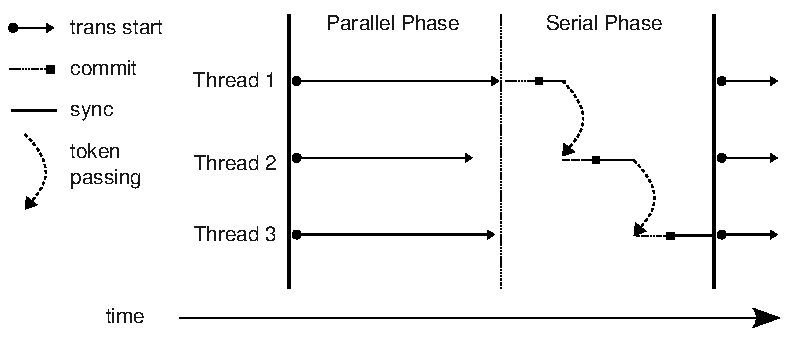
\includegraphics[width=6in]{dthreads/figure/phase}
\caption{An overview of \dthreads{} phase. Program execution with \dthreads{} alternates between parallel and serial phases.\label{fig:phase}}
}
\end{figure}

Figure~\ref{fig:phase} illustrates the execution of programs under \dthreads{}. \dthreads{} divides the execution of each thread into alternating parallel phases and serial phases. 
Based on the \sheriff{} framework, \dthreads{} isolates memory accesses in parallel phases. These accesses work on private copies of memory; that is, updates are not shared between threads during the parallel phases. When a synchronization point is reached, updates are applied (and made visible) in a deterministic order, as well as synchronizations. 
  
\subsection{Isolated Execution}
\label{sec:threadsasprocs}

Relying on the \sheriff{} framework, \dthreads{} turns threads into processes, with separate address spaces but the shared file table (Section~\ref{sec:threadcreat}). Thus, \dthreads{} isolates memory accesses among different threads between synchronization points: different threads can only see their own local changes. Those changes are merged together at synchronization points in order to achieve the shared memory semantics. 

\subsection{Deterministic Memory Commit}
\label{sec:sharedmem}

This section describes the mechanisms used to guarantee deterministic commits to the shared memory. These mechanisms are not provided by the \sheriff{} framework.   

\subsubsection{Fence and Token}
\label{sec:schedule}

\dthreads{} places internal fences between parallel and serial phases. \dthreads{} re-implements the fence because the standard \pthreads{}'s barrier mechanism does not support dynamic changes of threads number. 

\begin{figure}
\begin{lstlisting} [style=tt]
void waitFence(void) {
  lock();
	
  while(!isArrivalPhase()) { 
    CondWait();
  }

  waiting_threads++;
  if(waiting_threads < alive_threads) {
    while(!isDeparturePhase()) {
      CondWait();
    }
  } 
  else {
    setDeparturePhase();
    CondBroadcast();
  }

  waiting_threads--;
  if (waiting_threads == 0) {
    setArrivalPhase();
    CondBroadcast();
  }

  unlock();
}

\end{lstlisting}
\caption{Pseudocode for the internal fence.\label{fig:internalFence}}
\end{figure}

Figure~\ref{fig:internalFence} shows the pseudocode code for the internal fence. Threads must wait at an internal conditional variable until all threads depart from the last departure phase (lines 4-5). Then those threads are waiting at the fence until all alive threads have arrived at the same fence (lines 8-11). The last thread initiates the departure phase and wakes up all threads on the conditional variable (lines 14-15). As threads leave the fence, they decrement the number of waiting threads.  The last thread to leave sets the fence to the arrival phase and wakes any waiting threads (lines 19-21).

To reduce overhead, whenever the number of running threads is less than or equal to the number of cores, waiting threads use spin locks, instead of expensive cross-process \pthreads{} mutexes. When the number of threads exceeds the number of cores, \dthreads{} falls back to using \pthreads{} mutexes.

\begin{figure}
\begin{lstlisting} [style=tt]
void waitToken() {
  waitFence();
  while(isNotMyToken()) { yield(); }
}
void putToken() {
  passTokenToNextOfTokenQueue();
}
\end{lstlisting}
\caption{Pseudocode for waitToken and putToken. 
\label{fig:token}}
\end{figure}

Another key mechanism of \dthreads{} is the global token, which \dthreads{} uses to order memory commits and synchronizations. The token implementation is listed in Figure~\ref{fig:token}. The token is a shared pointer that points to the next runnable thread entry, which guarantees the global order for all operations in serial phases.  

\dthreads{} introduces two subroutines to manage tokens.  The \texttt{waitToken()} function first waits at the internal fence and then waits to acquire the global token in order to enter or leave the serial phases. The \texttt{putToken()} function passes the token to the next thread in the token-passing queue. 

As shown in Figure~\ref{fig:phase}, it is very important for a thread to wait at the internal fence before a thread enters or leaves serial phases, even for a thread that is guaranteed to have the token next. Otherwise, memory commits of a thread can affect other threads' behavior, bringing non-deterministic behavior for programs. 

\subsubsection{Commit Protocol}

Figure~\ref{fig:architecture} shows the steps to track modifications of every thread and expose them in a deterministic order.  

At the beginning of parallel phases, different threads have a read-only mapping for all shared pages. In parallel phases, if a thread writes to a page, this write is trapped in order to create a private copy and a identical twin page for this page. After that, reads and writes on this page happen on the private copy only. For those non-trapped pages, reads still go directly to the shared state.  

In serial phases, threads first commit their local changes that made in last parallel phase, guided by the global token.  The first thread  committing to a page can directly copy its private working copy to the shared state (page-based commits), but subsequent commits can only commit the modified bytes (byte-based commits), using the diffing and twinning mechanism discussed in Section~\ref{sec:twinning-and-diffing}. The byte-based commits are much slower than the page-based commits, but  they won't overwritten changes committed by those predecessors.  After a thread commits its local changes, it issues synchronizations before it passes the token to its next thread in the token-passing queue. 

In the end of serial phases, every thread has to release those private pages and twin pages, recover the read-only mapping, wait at the internal fence before entering into the next parallel phase. By removing those private pages and recovering those mappings, a thread is able to observe changes made by other threads, achieving the shared memory semantics. 

\subsection{Deterministic Synchronization}
\label{sec:synchronization}

\dthreads{} supports the full range of synchronizations of \pthreads{} library, including locks, conditional variables, barriers and different types of thread exits. Since the \sheriff{} framework can not provide any deterministic guarantee, \dthreads{} implements different types of synchronizations in a deterministic way as follows. 

\subsubsection{Locks}
Before a thread acquires a lock, it has to wait for the global token, by calling \texttt{waitToken}. 

\dthreads{} treats multiple locks as the same one. It only ends the current serial phase for a thread when all locks held by this thread are released. Because of that, it is possible for a program to avoid deadlock problems. 

At acquisitions of locks, \dthreads{} checks at first whether the current thread is already holding any locks. If not, the thread first waits for the token, commits those changes happened in the last parallel phase to the shared state, and begins a new atomic section. Then it increments the number of locks that it is currently holding before entering into critical sections. 

At deacquisitions of locks, \dthreads{} decrements the number of locks that the current thread holds first. A thread does nothing if it still holds some locks, with the number of locks not equal to 0. If all locks are released, \dthreads{} commits the memory changes made in this serial phase to the shared state. Then it passes the global token to the next thread in the token-passing queue, and waits on the internal fence before entering into the next round's parallel phase.

\subsubsection{Condition Variables}
\label{sec:condwait}

Guaranteeing determinism for condition variables is much more complex than for other synchronization primitives. The underlying operating system can not guarantee that threads are going to be waken-up in the same order as their waits. Thus, a naive implementation easily leads to a no-progress problem if the first waken-up thread can not get the global token to proceed first.

When a thread calls \texttt{pthread\_cond\_wait}, it first acquires the global token and commits local modifications made in the current serial phase since \texttt{pthread\_cond\_wait} is generally issued inside a critical section. It then removes itself from the token-passing queue, so that those threads waiting on condition variables do not participate in the token pass. Then, it adds itself to the conditional variable's waiting queue, decreases the number of alive threads (used in the internal fence mechanism), and passes the token to the next thread in the token-passing queue before actually waiting on a process-shared conditional variable. 

When a thread is awaken, it should check at first whether the current thread is ready to run or not. For a deterministic reason, \texttt{pthread\_cond\_signal} should only wake up the first thread waiting on a conditional variable and \texttt{pthread\_cond\_broadcast} wakes up all waiting threads. However, the underlying operating system, like Linux, can not guarantee this. To resolve this problem, in \texttt{pthread\_cond\_signal}, we specifically wake up all threads, but only the first thread is given the permission to run: If a thread is not able to run, it waits on this conditional variable again; If a thread is the candidate thread to be waken up, it waits for the global token to enter into the next serial phase; The candidate thread should get the token immediately in order to avoid a no-progress problem. 

For both \texttt{pthread\_cond\_signal} and \texttt{pthread\_cond\_broadcast}, the calling thread first waits for the global token, and then commits any local modifications before issuing an actual wake-up signal. When no threads are waiting on a condition variable, it passes the token to the next thread immediately, treating those calls as no-ops basically. Otherwise, it migrates corresponding threads, one for \texttt{pthread\_cond\_signal} and all for \texttt{pthread\_cond\_broadcast}, from the queue of this condition variable to the head of the token-passing queue, marks them as ready, increments the number of alive threads, and passes the token to the first thread in the token queue. 

\subsubsection{Barriers}

\label{sec:barrierwait}

Threads waiting on a barrier should not disrupt the token passing of running threads: \dthreads{} removes those waiting threads from the token-passing queue, and places them in corresponding barrier queue.

In order to ensure determinism, the calling thread first waits for the global token to commit any local modifications. If the current thread is the last one to enter the barrier, it moves all threads on the barrier queue to the token-passing queue, increases the number of alive threads, and passes the token to the first thread in the barrier queue. Otherwise, it removes itself from the token-passing queue, places itself in the barrier queue, releases the token, and waits on this actual barrier.


\subsubsection{Thread Creation and Exit}

\label{sec:threadcreation}

\begin{figure}
\begin{lstlisting} [style=tt]
void thread_create () {
  waitToken();
  clone(CLONE_FS| CLONE_FILES | CLONE_CHILD);
  if(isChild) {
    allocGlobalThreadIndex();
    insertToTokenQueue();
    notifyChildRegistered();
	// Wait for the parent to reach next sync point
    waitParentBroadcast();	
  }
  else if (isParent) {
    waitChildRegistered();
  }
}
\end{lstlisting}
\begin{lstlisting} [style=tt]
void thread_exit() {
  waitToken();
  atomicEnd(false);
  removeFromTokenQueue();
  decreaseInternalFence();
  putToken();
  exitThread(); 
}
\end{lstlisting}
\caption{Pseudocode for thread creation and exit($\S$~\ref{sec:threadcreation}).
\label{fig:threadcreation}
}
\end{figure}

To guarantee determinism, thread creations and exits must be performed in serial phases. 

In order to improve the parallelism and performance, a thread is allowed to create multiple threads without waiting for a new serial phase. Figure~\ref{fig:threadcreation} shows the pseudocode for thread creation and thread exit. First, the calling thread waits for the global token before proceeding (line 2). It then creates a new process, with shared file descriptors but a distinct address space, by invoking the \texttt{clone} system call (line 3).  Then the parent thread is waiting until its newly spawned child has registered itself. 

The newly spawned child obtains the global thread index (line 5), places itself in the token-passing queue (line 6), and notifies the parent that registration has finished(line 7). Then it waits for the notification from the parent to proceed when the parent to reach the next synchronization point, not a thread creation.  In this way, we can allow a parent thread to create multiple children threads in the same serial phase. 

When \texttt{thread\_exit()} is called, the caller first waits for the global token before committing any local modifications (line 3). It then removes itself from the token-passing queue (line 4), and decreases the number of alive threads (line 5). Finally, it passes the gobal token to the next thread in the token queue (line 6) and exits (line 7).

\subsubsection{Thread Cancellation}

\dthreads{} performs thread cancellations in serial phases for the deterministic reason. A thread can only invoke \texttt{pthread\_cancel} while holding the global token. If the thread being cancelled is waiting on a condition variable or a barrier, it is removed from the queue deterministically. Finally, to cancel a thread, \dthreads{} kills the target process using kill(tid, SIGKILL) and decrements the number of alive threads after the cancellation.

\subsection{Deterministic Memory Allocation}
Sometimes, programs may rely on the addresses of objects returned by the memory allocator intentionally (for example, by hashing objects based on their addresses), or accidentally. A program with a memory error, like a buffer overflow, will yield different results for different memory layouts.

The reliance on memory addresses can undermine other efforts to provide determinism. For example, CoreDet is unable to fully enforce determinism because it relies on the Hoard scalable memory allocator~\cite{Bergan:2010:CCR:1736020.1736029}. Hoard was not designed to provide determinism and several of its mechanisms, thread id based hashing and non-deterministic assignment of memory to threads, lead to nondeterministic execution in CoreDet for the Canneal benchmark. To resolve this problem, \dthreads{} employs both deterministic thread index and custom memory allocation mechanism. 

\subsubsection{Deterministic Thread Index}
\label{sec:threadindex}

POSIX does not guarantee deterministic process or thread identifiers. To avoid exposing this nondeterminism to threads that run as processes, \dthreads{} shims \texttt{pthread\_self()} in order to return a deterministic thread index on different executions. This thread index is managed using a single global variable that is incremented on every thread creation.  This unique thread index is also used to manage per-thread heaps and as an index into an array of thread entries.

\subsubsection{Custom Memory Allocation}

To preserve determinism in the face of intentional or inadvertent reliance on memory addresses, we designed the \dthreads{} memory allocator to be fully deterministic. 

\dthreads{} assigns subheaps to each thread based on its deterministically assigned thread index. In addition to guarantee the same mapping of threads to subheaps on different executions, \dthreads{} allocates superblocks (large chunks of memory) deterministically by acquiring a lock (under the global token) on each superblock allocation. Thus, threads always use the same subheaps, and these subheaps always acquires the same superblocks on each execution. The superblocks themselves are allocated via mmap: while \dthreads{} could use a fixed address mapping for the heap, we currently simply disable ASLR to provide deterministic mapping from mmap calls. If a program does not rely on absolute addresses, \dthreads{} can guarantee determinism even with ASLR enabled. However, hash functions and lock-free algorithms frequently use absolute addresses, and any deterministic multithreading system must disable ASLR to provide deterministic results for these cases.


\section{Optimizations}
\label{sec:dthreads-optimization}

\dthreads{} performs a number of optimizations to improve its performance.

\textbf{Lazy commit:} \dthreads{} reduces its copying overhead and the time spent in serial phases by lazily committing pages. When only one thread has ever modified a page, \dthreads{} considers this thread to be the owner of this page. An owned page is committed to the shared state only when another thread attempts to read or write this page. \dthreads{} tracks accesses from other threads using page protection, and signals the owning thread to commit pages on demand. To reduce the number of read faults, pages holding global variables (which we expect to be shared) and any pages in the heap that have ever had multiple writers are all considered unowned and are not read-protected.

\textbf{Single-threaded-execution: }
When only one thread is running, \dthreads{} does not enable memory protection and treats all synchronization operations as no-ops. In addition, when only one thread is active and other threads are waiting on conditional variables, \dthreads{} does not commit local changes to the shared mapping (and discard private dirty pages). Updates are only committed when the current thread issues a \texttt{cond\_signal} or \texttt{cond\_broadcast} call, which can wake up other threads and thus require publication of all updates made by this thread.

\textbf{Lazy twin creation and diff elimination: }
To further reduce \dthreads{}'s copying and memory overhead, twin pages are only created for those pages that have multiple writers during the same transaction. In commit phases, a single writer of a page can directly copy its private working page to shared state, without performing a byte-by-byte comparison. Thus, when one thread is the sole writer of a page, this optimization saves a page allocation and a page copy during the execution (either parallel phases or serial phases), and a comparison in commit phases.
In addition, \dthreads{} eliminates unnecessary comparisons for all first committers, by associating a global version number (incremented at each commit) for every dirty page: In the page fault handler, every thread gets a local version number for current dirty page additionally; A thread can directly copies its working copy for each page whenever its local version number equals its global version number, since this thread is the first committer on this page and there is only one thread that can commit at a time in serial phases.  

\textbf{Lock ownership:} \dthreads{} uses lock ownership to avoid unnecessary waiting when threads are using distinct locks. Initially, all locks are unowned. Any thread attempting to acquire a lock that it does not own must wait until a serial phase to do so. If multiple threads attempt to acquire the same lock, this lock is marked as ``shared''. If only one thread attempts to acquire a lock, this thread takes the ownership of this lock and can acquire and release it during parallel phases. Lock ownership can result in starvation if a thread continues to re-acquire an owned lock without entering serial phases, while other threads are aiming to acquire the same lock (and waiting on the fence). To avoid this problem, each lock has a maximum number of times that it can be acquired during a parallel phase before a serial phase is required.

\textbf{Parallelization: }
\dthreads{} attempts to exploit as much parallelism as possible in the runtime system. One optimization is that at the start of transactions, \dthreads{} performs certain cleanup tasks, including releasing private page frames or resetting pages to a read-only mode. It is safe to perform these cleanup tasks concurrently since these operations do not affect other threads's behavior.
Thus, \dthreads{} parallelizes a thread's cleanup tasks with other threads’ commit operations, without holding the global token. With this optimization, the token is passed to the next thread as soon as possible, reducing time in serial phases. 

\section{Evaluation}
\label{sec:dthreadsevaluation}

We perform our evaluation on an Intel Core 2 dual-processor CPU system, equipping with 16GB of RAM. Each processor is a 4-core 64-bit Xeon, running at 2.33GHZ with a 4MB L2 cache. The operating system is an unmodified CentOS 5.5, running with Linux kernel version 2.6.18-194.17.1.el5.

\subsection{Methodology}

We evaluate the performance and scalability of \dthreads{} (versus CoreDet and \pthreads{}) across the PARSEC~\cite{parsec} and Phoenix~\cite{phoenix-hpca} benchmark suites.  

In order to compare performance directly against CoreDet, which relies on the LLVM infrastructure~\cite{LLVM:CGO04}, all benchmarks are compiled with the LLVM compiler at the ``-O3'' optimization level~\cite{LLVM:CGO04}. Since \dthreads{} does not currently support 64-bit binaries, all benchmarks are compiled for 32 bit environments (using the ``-m32'' compiler flag). Each benchmark is executed ten times on a quiescent machine. To reduce the effect of outliers, results with the worst and best performance for each benchmark are discarded,
so each result is the average of the remaining eight runs.

\textbf{Tuning CoreDet:} 
The performance of CoreDet~\cite{Bergan:2010:CCR:1736020.1736029} is extremely sensitive to three parameters: the granularity for the ownership table (in bytes), the quantum size (in number of instructions retired), and the choice between full serial mode and reduced serial mode. We compare the performance and scalability of \dthreads{} with the best possible results that we could obtain for CoreDet on our system---that is, with the lowest average normalized
runtime---after an extensive search of the parameter space (six possible granularities and 8 possible quanta, for each benchmark). The results presented here are for a 64-byte granularity, a quantum size of 100,000 instructions, and in full serial mode.

\textbf{Unsupported Benchmarks}: We do not include results for 7 benchmarks from PARSEC, since they do not currently work with \dthreads{} (note that many of these also do not work for CoreDet). \texttt{vips} and \texttt{raytrace} would not build as 32-bit executables; \texttt{bodytrack}, \texttt{facesim}, and \texttt{x264} depend on sharing of stack variables;
\texttt{fluidanimate} uses ad-hoc synchronization, so it cannot run without modifications; and \texttt{freqmine} does not use \pthreads{}.

 
\textbf{Scalability Experiment}: For all scalability experiments, we logically disable CPUs using Linux's CPU hotplug mechanism, which allows us to disable or enable a specific CPU by writing ``0'' or ``1'' to a file: \texttt{/sys/devices/system/cpu/cpuN/online}.

\subsection{Determinism}

We first experimentally verify \dthreads{}' ability to ensure determinism by executing the \emph{racey} determinism tester~\cite{1508256}. This stress test contains, as its name suggests, numerous data races and is thus extremely sensitive to memory-level non-determinism. \dthreads{} reports the same results for 2,000 runs. We also verify that the schedules and outputs of all benchmarks of every execution are identical.

\subsection{Performance}
\label{sec:performance}

\begin{figure*}[!t]
{\centering
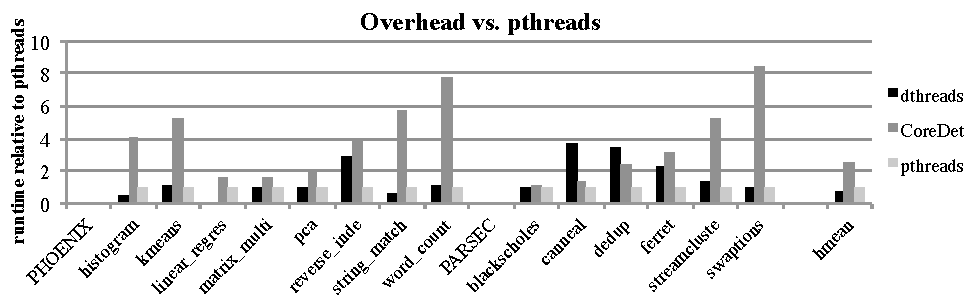
\includegraphics[width=6in]{dthreads/figure/overhead-figure}
\caption{Normalized execution time with respect to \pthreads{} and CoreDet(lower is better). For 9 of the 14 benchmarks, \dthreads{} runs nearly as fast or faster than \pthreads{}, while providing deterministic behavior.\label{fig:performance}}
}
\end{figure*}

\begin{table*}[!t]
\centering
\resizebox{\columnwidth}{!}{
\begin{tabular}{l|rr|l}
{\bf \small Benchmark} & $\frac{\mbox{\bf \small CoreDet}}{\mbox{\bf \small \pthreads{}}}$ & $\frac{\mbox{\small \bf \dthreads{}}}{\mbox{\small \bf \pthreads{}}}$ & {\bf \small Input} \\

\hline
{\bf \small histogram} &  $4.35\times$ & $0.52\times$ & {\it \small large.bmp} \\
{\bf \small kmeans} &  $5.05\times$ & $0.91\times$ & {\it \small -d 3 -c 1000 -p 100000 -s 1000} \\ 
{\bf \small linear\_regression}  & $1.50\times$ & $0.13\times$ & {\it \small key\_file\_500MB.txt} \\
{\bf \small matrix\_multiply}  & $1.55\times$ & $1.00\times$ & {\it \small 2000 2000 } \\
{\bf \small pca}  & $1.94\times$ & $1.03\times$ & {\it \small -r 4000 -c 4000 -s 100 } \\
{\bf \small reverse\_index} & $4.64\times$ & $2.73\times$ & {\it \small datafiles} \\
{\bf \small string\_match} & $5.95\times$ & $0.65\times$ & {\it \small key\_file\_500MB.txt} \\
{\bf \small word\_count} & $7.67\times$ & $1.09\times$ & {\it \small word\_100MB.txt} \\
{\bf \small blackscholes} & $1.13\times$ & $0.98\times$ & {\it \small 8 in\_1M.txt prices.txt} \\
{\bf \small canneal} & $1.00\times$ & $4.12\times$ &  {\it \small 7 15000 2000 400000.nets 128} \\
{\bf \small dedup} & $2.69\times$ & $3.39\times$ & {\it \small -c -p -f -t 2 -i media.dat output.txt} \\
{\bf \small ferret} & $3.69\times$ & $2.84\times$ & {\it \small corel lsh queries 10 20 1 output.txt} \\
{\bf \small streamcluster} & $4.87\times$ & $1.44\times$ &  {\it \small 10 20 128 16384 16384 1000 none output.txt 8} \\
{\bf \small swaptions} & $7.61\times$ & $0.95\times$ & {\it \small -ns 128 -sm 50000 -nt 8} \\
\hline
\end{tabular}
}
\caption{Benchmarks: normalized execution time and input parameters.\label{tbl:benchmarks}}
\end{table*}

For performance, We compare \dthreads{} to CoreDet
and \pthreads{}. Figure~\ref{fig:performance} presents these results graphically (normalized to the runtime of \pthreads{}); Table~\ref{tbl:benchmarks} provides detailed information about the normalized execution time and input parameters.

\dthreads{} outperforms CoreDet on 12 out of 14 benchmarks (running between 20\% and $12\times$ faster). For 9 benchmarks, \dthreads{} runs nearly the same as or better
performance than \texttt{pthreads}. Because \dthreads{} isolates updates in separate processes, it can improve performance by eliminating false sharing: since concurrent ``threads'' actually perform at different physical pages, there is no coherence traffic caused by false sharing between synchronization points. \dthreads{} eliminates catastrophic false sharing in the \texttt{linear\_regression} benchmark, allowing it to execute over $8\times$ faster than \pthreads{} and $12\times$ faster than CoreDet. The \texttt{string\_match} benchmark exhibits a similar, though less dramatic, false sharing problem, allowing \dthreads{} to run almost 56\% faster than \pthreads{} and $9\times$ faster than CoreDet. Two benchmarks, \texttt{histogram} and \texttt{swaptions}, also run faster with \dthreads{} than with \pthreads{} ($2\times$ and $6\%$, respectively; $2.7\times$ and $9\times$ faster than with CoreDet). We believe but have not yet verified that the reason is false sharing.

\dthreads{} runs substantially slower than \pthreads{} for 4 of the 14 benchmarks examined here. The \texttt{ferret} benchmark relies on an external library to analyze image files during the first stage in its pipelined execution model; this library makes intensive (and in the case of \dthreads{}, unnecessary) use of locks. Lock acquisitions and deacquisitions in \dthreads{} imposes higher overhead than ordinary \pthreads{} mutex operations. More importantly in this case, the intensive use of locks in one stage forces \dthreads{} to effectively serialize the other stages in the pipeline, which must repeatedly wait on these locks to enforce a deterministic lock acquisition order. The other three benchmarks (\texttt{canneal}, \texttt{dedup}, and \texttt{reverse\_index}) modify a large number of pages. With \dthreads{}, each page modification triggers a segmentation violation, a system call to change memory protection, the creation of a private copy of the page, and a subsequent copy into the shared space during commit phases. We note that CoreDet also substantially degrades performance for \texttt{dedup} and \texttt{reverse\_index}), so much of this slowdown may be inherent to any deterministic runtime system.

\subsection{Scalability}
\label{sec:scalability}

\begin{figure}
{\centering
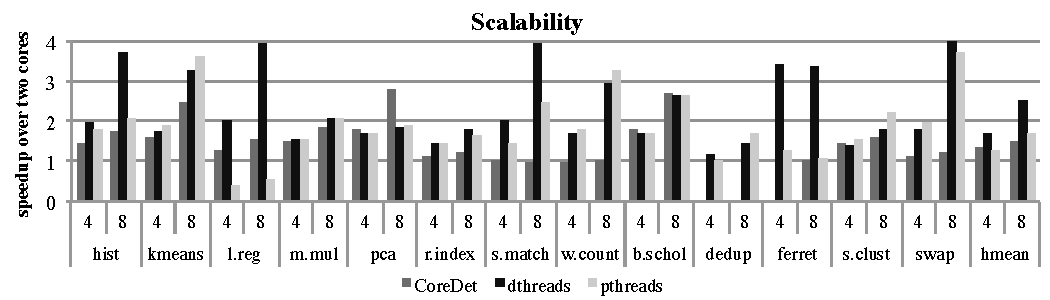
\includegraphics[width=6in]{dthreads/figure/scalability-figure}
\caption{Speedup of eight cores versus two cores (higher is better).  When possible to control with command line options, the number of threads was matched to the number of cores enabled.\label{fig:scalability}}
}
\end{figure}

To measure the scalability cost of running \dthreads{}, we ran two benchmark suite (excluding \texttt{canneal}) on the same machine with eight cores and again with two cores enabled.  Whenever possible without source code modifications, the number of threads was matched to the number of CPUs enabled.  We have found that \dthreads{} scales at least as well as \pthreads{} for 9 of 13 benchmarks, and scales as well or better than CoreDet for all but one benchmark where \dthreads{} outperforms CoreDet by 2x.  Detailed results of this experiment are presented in Figure~\ref{fig:scalability} and discussed below.

\texttt{canneal} was excluded from the scalability experiment because this benchmark does more work when more threads are present, making the performance comparison between eight and two threads unfair.  \dthreads{} hurts scalability relative to \pthreads{} for four of the benchmarks: \texttt{kmeans}, \texttt{word\_count}, \texttt{dedup}, and \texttt{streamcluster} although only marginally in most cases.  In all of these cases, \dthreads{} scales better than CoreDet.

\dthreads{} is able to match the scalability of \pthreads{} for three benchmarks: \texttt{matrix\_multiply}, \texttt{pca}, and \texttt{blackscholes}.  With \dthreads{}, scalability actually \emph{improves} over \pthreads{} for 6 out of 13 benchmarks: \texttt{histogram}, \texttt{linear\_regression}, \texttt{reverse\_index}, \texttt{string\_match}, \texttt{ferret}, and \texttt{swaptions}.




\subsection{Performance Analysis}

\subsubsection{Benchmark Characteristics}

The data presented in Table~\ref{tbl:characteristics} are obtained from the executions running on all 8 cores.  Column 2 shows the percentage of time spent in serial phases.  In \dthreads{}, all memory commits and actual synchronization operations are performed in serial phases.  The percentage of time spent in serial phases thus can affect performance and scalability. Applications with higher overhead in \dthreads{} often spend a higher percentage of time in
serial phases, primarily because they modify a large number of pages that need to be committed during serial phases.

Column 3 shows the number of transactions in each application and Column 4 provides the average length of each transaction (ms).  Every synchronization, including locks, conditional variable, barriers, and thread exits, demarcate transaction boundaries in \dthreads{}.  For example, \texttt{reverse\_index}, \texttt{dedup}, \texttt{ferret}
and \texttt{streamcluster} perform numerous transactions whose
execution time is less than 1ms, imposing a performance penalty for these applications.  Benchmarks with longer (or fewer) transactions run almost the same speed as or faster than \texttt{pthreads}, including \texttt{histogram} or \texttt{pca}.  In \dthreads{}, longer transactions amortize the overhead of memory protection and copying over a longer period, thus reducing performance overhead.

Column 5 and 6 provides more detail on the costs associated with memory updates (the number and total volume of dirtied pages). From the table, it is clear why \texttt{canneal} (the most notable outlier) runs much slower with \dthreads{} than with \pthreads{}. This benchmark updates over three million pages, leading to large performance overhead caused by creating private copies, handling protection faults, and committing modifications on those pages to the shared memory mapping. 

\textbf{Conclusion: }
Most benchmarks examined here contain either a small number of transactions, thus having long running transactions, and modify a modest number of pages during execution. For these applications, \dthreads{} is able to amortize its overhead: by eliminating false sharing, it can even run faster than \pthreads{}. However, for the few benchmarks that perform numerous short-lived transactions, or modify a large amount of pages, \dthreads{} can introduce substantial overhead.


\begin{table*}[!t]
\centering
\resizebox{\columnwidth}{!}{
\begin{tabular}{l|rrrrr}
& {\bf \small Serial Phase} & {\bf \small Transactions} & {\bf \small TransLength} & {\bf \small DirtyPages} & {\bf \small DirtyPages}
\\
{\bf \small Benchmark} & {\bf \small (\% of time)} & {\bf (\#)} & {\bf \small (ms)} & {\bf \small (\#)} & {\bf \small (GB)}\\
%\hline
%\multicolumn{6}{|c|}{\emph{Phoenix}} \\
\hline
\small \textbf{histogram} & 0 & 23 & 15.47 & 29 & 0 \\
\small \textbf{kmeans} & 0 & 3929 & 3.82 & 9466 & 0.04\\
\small \textbf{linear\_regression} & 0 & 24 & 23.92 & 17 & 0\\
\small \textbf{matrix\_multiply} & 0 & 24 & 841.2 & 3945 & 0.02\\
\small \textbf{pca} & 0 & 48 & 443 & 11471 & 0.04 \\
\small \textbf{reverseindex} & 17\% & 61009 & 1.04 & 451876 & 1.72\\
\small \textbf{string\_match} & 0 & 24 & 82 & 41 & 0 \\
\small \textbf{word\_count} & 1\% & 90 & 26.5 & 5261 & 0.02\\
%\hline
%\multicolumn{6}{|c|}{\emph{PARSEC}} \\
%\hline
\small \textbf{blackscholes} & 0 & 24 & 386.9 & 991 & 0\\
\small \textbf{canneal} & 26.4\% & 1062 & 43 & 3606413 & 13.75\\
\small \textbf{dedup} & 31\% & 45689 & 0.1 & 356589 & 1.36\\
\small \textbf{ferret} & 12.3\% & 484127 & 0.05 & 844184 & 3.21 \\
\small \textbf{streamcluster} & 18.4\% & 130001 & 0.04 & 131992 & 0.50\\
\small \textbf{swaptions} & 0 & 24 & 163 & 867 & 0\\
\hline
\end{tabular}
}
\caption{Benchmark characteristics.\label{tbl:characteristics}}
\end{table*}

\subsubsection{Performance Impact Analysis}
We further evaluate the performance impact of two important components of \dthreads: deterministic synchronization (sync-only) and memory protection(prot-only).

\emph{Sync-only}: This configuration enforces a deterministic synchronization order. However, memory protection is not enabled so all ``threads'' (actually processes) access the shared memory directly. We want to use this to show the performance impact of load imbalance, caused by synchronization based scheduling.

\emph{Prot-only}: This configuration runs threads in isolation, and commits at synchronization points. The order of synchronization and memory commits are non-deterministic. This configuration eliminates false sharing, but also introduces the performance overhead of isolation and memory commits. In order to guarantee correct execution, we replaced those synchronizations as corresponding cross-processes synchronizations. The lazy twin creation and single-threaded execution optimizations are disabled here because they are unsafe without deterministic synchronization. Thus, this configuration actually evaluates the performance of the \sheriff{} framework. 


\begin{figure*}[!t]
{\centering
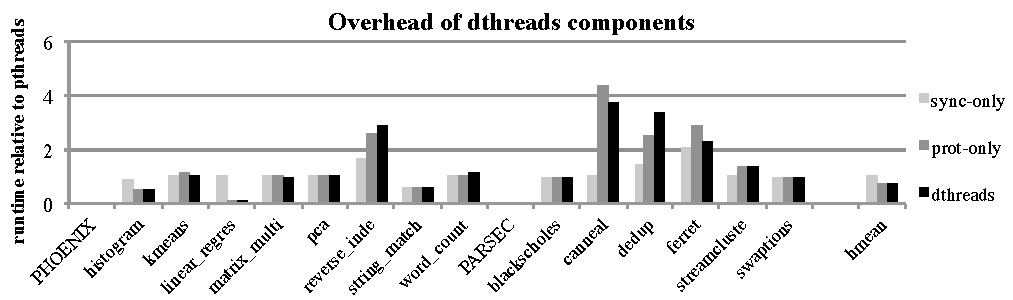
\includegraphics[width=6in]{dthreads/figure/perfeffect}
\caption{Normalized execution time with respect to \pthreads{} (lower is better) for three different configurations. 
\label{fig:perfanalysis}}
}
\end{figure*}

The performance results of these two configurations are shown in Figure~\ref{fig:perfanalysis} and discussed in the following.

\begin{itemize}

\item
The \texttt{reverse\_index}, \texttt{dedup} and \texttt{ferret} benchmarks show significant load imbalance under {\it sync-only} configuration. Additionally, these benchmarks introduces significant overhead with {\it prot-only} configuration because of a large number of transactions there. That explains why \dthreads{} doesn't have good performance on these benchmarks.

\item
The \texttt{string\_match} benchmark shows performance improvement with {\it sync-only} configuration. The exact reason is not clear, may be due to our custom memory allocator (described in Section~\ref{sec:customheap}) that eliminates false sharing problems. 

\item
The \texttt{linear\_regression}, \texttt{histogram} and \texttt{swaptions} benchmarks improve performance with {\it prot-only} configuration. The memory isolation mechanism eliminates false sharing problems inside and contributes to the performance speedup.

\item
Normally the performance of \dthreads{} is not better than the performance of the {\it prot-only} configuration. However, both \texttt{ferret} and \texttt{canneal} run faster with determinism enabled (under \dthreads{}). Both are benefited from specific optimization described in Section~\ref{sec:dthreads-optimization}. \texttt{ferret} benefits from the \emph{single-threaded-execution}. The performance improvement of \texttt{canneal} is coming from the shared twin pages for all threads in parallel phases.

\end{itemize}







\section{Discussion}
\label{sec:discussion} All DMT systems must impose an order on updates to shared memory and synchronization operations.  The
mechanism used to isolate updates affects the limitations and performance of the
system.  \dthreads{} represents a new point in the design space for DMT systems with some inherent advantages and limitations as follows.

\subsection{Design Tradeoffs} 

CoreDet and \dthreads{} both use a combination of
parallel and serial phases to execute programs deterministically.  These two systems take different approaches during parallel phases, as
well as the transitions between phases:

\textbf{Memory isolation:} 
CoreDet orders updates to the shared memory by
instrumenting all memory accesses that could reference shared data. Synchronization operations and updates to shared memory must be performed in serial phases, unless those updates are performed by owners of a block, which can issued in parallel phases. This approach results in high instrumentation overhead during parallel phases, but incurs no additional overhead when exposing updates to the shared state since they are shared already.

\dthreads{} takes an alternate approach: updates proceed at full speed, but are isolated using hardware-supported virtual memory.  When a serial phase is reached, these updates are committed to the shared state in a deterministic order, with
the help of the twinning and diffing mechanism described in Section~\ref{sec:twinning-and-diffing}.

A pleasant side-effect of \dthreads{} is the elimination of false sharing. Because threads work in separate address spaces, there is no need to keep caches coherent between threads during parallel phases.  For some programs, this results in a performance improvement as large as $7\times$ when compared to
\pthreads{}.

\textbf{Phases:} 
CoreDet employs a quantum-based scheduler: after the specified number of instructions is executed in a parallel phase, the scheduler transitions to a serial phase. This approach bounds the waiting time for any thread that are blocked to the quantum, reducing the load imbalance problem.  One drawback of this approach is that transitions to a serial phase do not correspond to static program points.  Any changes of code and input will result in a new, previously-untested schedule.

Transitions between phases are static in \dthreads{}.  Any synchronization operation will result in a transition to a serial phase, and a parallel phase
will resume once all threads have finished their critical sections.  This makes \dthreads{} susceptible to delays due to load imbalance between threads, but results in more robust determinism.  With \dthreads{}, only the order of synchronization operations affects the schedule. For most programs, this means that different inputs, and even many code changes, will not change the schedule produced by \dthreads{}, as long as those changes won't affect the order of synchronizations.

\subsection{Limitations}
\label{sec:limitations}

This section analyzes some key limitations of \dthreads{} that restrict its ability to run certain programs, limit the extent of determinism it can guarantee, or potentially affect performance.

\textbf{Unsupported programs: }
\dthreads{} supports programs that
use the pthreads library, but does not support programs that
bypass it by using their own ad hoc synchronization operations, such as those that use atomic operations. However, the upcoming C++0X standard includes a library interface for atomic operations~\cite[pp. 1107--1128]{c++0xstandarddraft}, and a future version of \dthreads{} could intercept these library calls and treat them as synchronization points. While ad hoc synchronization is a common practice, it is also a notorious source of bugs; Xiong et al.\ show that 22--67\% of the uses of ad hoc
synchronization lead to bugs or severe performance issues~\cite{ad-hoc-considered-harmful}.

Currently, \dthreads{} also does not share the stack
across threads, so any updates to stack variables are only locally visible, which could cause a program to fail. However, communicating across different threads using stack variables  is extremely error-prone and generally deprecated, making this a rare coding practice.

\textbf{External determinism: }
While \dthreads{} provides internal determinism, it does not guarantee determinism when a program's behavior depends on external sources of non-determinism, such as system time or I/O events. Incorporation of \dthreads{} in the dOS framework, an OS proposal that enforces system-level determinism, would provide full deterministic execution, although this remains future work~\cite{deterministic-process-groups}.

\textbf{Runtime performance: }
Section~\ref{sec:evaluation} shows that \dthreads{} can provide high performance for a number of applications; in fact, for the majority of the benchmarks examined, \dthreads{} matches or even exceeds the performance of \pthreads{}. However, \dthreads{} could occasionally degrade performance, sometimes substantially. One way it could do so would be to exhibit an intensive use of locks (that is, acquiring and releasing locks at very high frequency), which are much more expensive
in \dthreads{} than in \pthreads{}. However, because of its determinism guarantees, \dthreads{} could allow programmers to greatly reduce their use of locks, and thus improve performance. Other application characteristics, also explored in Section~\ref{sec:performance}, can also impair performance
with \dthreads{}.


%  Since Surprise locking inside libraries. Not a limitation \emph{per
%  se} but definitely an issue that could surprise programmers.

% Draft can be downloaded from http://www.open-std.org/jtc1/sc22/wg21/docs/papers/2010/n3126.pdf.
%Fine once they are library calls, as they are in gcc and in the upcoming C++0X standard (cite!), since then we can intercept them.

\textbf{Memory consumption: }
Because \dthreads{} creates private, per-process copies of modified pages between commits, it can increase a program's memory footprint by the number of modified pages between synchronization points. This increased footprint does not seem to be a problem in practice, both because the number of modified pages is generally far smaller than the number of pages read, and because it is transitory: all private pages are relinquished to the operating system (via \texttt{madvise()}) at the end of every commit operation.

\textbf{Memory consistency:} 
\dthreads{} provides a form of release consistency for parallel programs, where updates are exposed at static program points. 
CoreDet's DMP-B mode also uses release consistency, but the update points depend on when the quantum counter reaches zero.  To the best of our knowledge, \dthreads{} cannot produce an output that is not possible with \pthreads{}, although for some cases it will result in unexpected outputs.  But the same unexpected output will be produced on every run
with \dthreads{}, making it easier for developers to track down the source of the problem than with \pthreads{}.


